\documentclass[10pt,landscape]{article}
\usepackage{multicol}
\usepackage{calc}
\usepackage{ifthen}
\usepackage[landscape]{geometry}
\usepackage{graphicx}
\usepackage{amsmath, amssymb, amsthm}
\usepackage{latexsym, marvosym}
\usepackage{pifont}
\usepackage{lscape}
\usepackage{graphicx}
\usepackage{lipsum}
\usepackage{array}
\usepackage{booktabs}
\usepackage[bottom]{footmisc}
\usepackage{tikz}
\usetikzlibrary{shapes}
\usepackage{pdfpages}
\usepackage{wrapfig}
\usepackage{enumitem}
\setlist[description]{leftmargin=0pt}
\usepackage{xfrac}
\usepackage[pdftex,
            pdfauthor={Pablo Angulo},
            pdftitle={python and MILP Cheatsheet},
            pdfsubject={A cheatsheet pdf and reference guide covering basic python commands and basic MILP theory by Pablo Angulo for ETSIN@UPM},
            pdfkeywords={python} {programming} {MILP} {optimization} {optlang} {numpy} {pdf} {cheat} {sheet}
            ]{hyperref}
\usepackage[
            open,
            openlevel=2
            ]{bookmark}
\usepackage{relsize}
\usepackage{rotating}

\usepackage{color}
\definecolor{gray95}{gray}{.95}
\definecolor{gray75}{gray}{.75}
\definecolor{gray45}{gray}{.45}

\usepackage{listings}
\definecolor{keywords}{RGB}{48,48,255}
\definecolor{comments}{RGB}{70,180,130}
\definecolor{strings}{RGB}{30,200,60}
\definecolor{gray95}{RGB}{245,245,245}
\lstset{ frame=Ltb,
     framerule=0pt,
     aboveskip=0.3cm,
     framextopmargin=1.5pt,
     framexbottommargin=1.5pt,
     framexleftmargin=0.3cm,
     framesep=0pt,
     rulesep=0pt,
%     backgroundcolor=\color{gray95},
     rulesepcolor=\color{black},
     %
     stringstyle=\ttfamily,
     showstringspaces = false,
     basicstyle=\scriptsize\ttfamily,
     commentstyle=\color{comments}\emph,
     keywordstyle=\bfseries\color{keywords},
     stringstyle=\color{strings},
     %
     numbers=none,
     numbersep=12pt,
     numberstyle=\tiny,
     numberfirstline = false,
     breaklines=true,
	%
	language=Python
	}

% minimizar fragmentado de listados
\lstnewenvironment{listing}[1][]
   {\lstset{#1}\pagebreak[0]}{\pagebreak[0]}

\lstdefinestyle{consola}
   {basicstyle=\scriptsize\bf\ttfamily,
    backgroundcolor=\color{gray75},
   }


 \newcommand\independent{\protect\mathpalette{\protect\independenT}{\perp}}
    \def\independenT#1#2{\mathrel{\setbox0\hbox{$#1#2$}%
    \copy0\kern-\wd0\mkern4mu\box0}}

\newcommand{\R}{\mathbb{R}}
\newcommand{\noin}{\noindent}
\newcommand{\logit}{\textrm{logit}}
\newcommand{\var}{\textrm{Var}}
\newcommand{\cov}{\textrm{Cov}}
\newcommand{\corr}{\textrm{Corr}}
\newcommand{\N}{\mathcal{N}}
\newcommand{\DisUniform}{\textrm{DisUniform}}
\newcommand{\Bern}{\textrm{Bern}}
\newcommand{\Bin}{\textrm{Bin}}
\newcommand{\Beta}{\textrm{Beta}}
\newcommand{\Gam}{\textrm{Gamma}}
\newcommand{\IGam}{\textrm{InverseGamma}}
\newcommand{\Expo}{\textrm{Expo}}
\newcommand{\Pois}{\textrm{Pois}}
\newcommand{\Unif}{\textrm{Unif}}
\newcommand{\Geom}{\textrm{Geom}}
\newcommand{\NBin}{\textrm{NBin}}
\newcommand{\Hypergeometric}{\textrm{HGeom}}
\newcommand{\HGeom}{\textrm{HGeom}}
\newcommand{\Mult}{\textrm{Mult}}

\geometry{top=.4in,left=.2in,right=.2in,bottom=.4in}

\pagestyle{empty}
\makeatletter
\renewcommand{\section}{\@startsection{section}{1}{0mm}%
                                {-1ex plus -.5ex minus -.2ex}%
                                {0.5ex plus .2ex}%x
                                {\normalfont\large\bfseries}}
\renewcommand{\subsection}{\@startsection{subsection}{2}{0mm}%
                                {-1explus -.5ex minus -.2ex}%
                                {0.5ex plus .2ex}%
                                {\normalfont\normalsize\bfseries}}
\renewcommand{\subsubsection}{\@startsection{subsubsection}{3}{0mm}%
                                {-1ex plus -.5ex minus -.2ex}%
                                {1ex plus .2ex}%
                                {\normalfont\small\bfseries}}
\makeatother

\setcounter{secnumdepth}{0}

\setlength{\parindent}{0pt}
\setlength{\parskip}{0pt plus 0.5ex}

% -----------------------------------------------------------------------

\usepackage{titlesec}

\titleformat{\section}
{\color{blue}\normalfont\large\bfseries}
{\color{blue}\thesection}{1em}{}
\titleformat{\subsection}
{\color{cyan}\normalfont\normalsize\bfseries}
{\color{cyan}\thesection}{1em}{}
% Comment out the above 5 lines for black and white

\begin{document}

\raggedright
\footnotesize
\begin{multicols*}{3}

% multicol parameters
% These lengths are set only within the two main columns
%\setlength{\columnseprule}{0.25pt}
\setlength{\premulticols}{1pt}
\setlength{\postmulticols}{1pt}
\setlength{\multicolsep}{1pt}
\setlength{\columnsep}{2pt}

%%%%%%%%%%%%%%%%%%%%%%%%%%%%%%%%%%%%
%%% TITLE
%%%%%%%%%%%%%%%%%%%%%%%%%%%%%%%%%%%%

\begin{center}
    {\color{blue} \Large{\textbf{Python and MILP Cheatsheet}}} \\
   % {\Large{\textbf{Probability Cheatsheet}}} \\
    % comment out line with \color{blue} and uncomment above line for b&w
\end{center}

%%%%%%%%%%%%%%%%%%%%%%%%%%%%%%%%%%%%
%%% ATTRIBUTIONS
%%%%%%%%%%%%%%%%%%%%%%%%%%%%%%%%%%%%

\scriptsize

Pablo Angulo for ESTIN@UPM.ES

% \begin{center}
%     Last Updated \today
% \end{center}

% Cheatsheet format from
% http://www.stdout.org/$\sim$winston/latex/

%%%%%%%%%%%%%%%%%%%%%%%%%%%%%%%%%%%%
%%% BEGIN CHEATSHEET
%%%%%%%%%%%%%%%%%%%%%%%%%%%%%%%%%%%%


\section{\texttt{python}}\smallskip \hrule height 2pt \smallskip
\subsection{Base types}

\begin{description}
  \item[\texttt{bool}] \emph{booleans} takes only two values: \texttt{True} and \texttt{False}.
  \item[\texttt{int}] positive and negative \emph{integers}, not bounded
  \item[\texttt{float}] \emph{floating point} numbers approximate any real number (e.g. \texttt{-1.25e-6} ($-1.26\cdot 10^{-6}$))
  \item[\texttt{str}] A \emph{string} is a sequence of characters. Always represented with quotes or double quotes (e.g. \texttt{'Hello, World'}, or \texttt{"Hello, World"})
\end{description}

\subsection{Variables}
\emph{Identifiers} start with a letter or \texttt{\_}, may contain numbers.

\texttt{identifier = value} binds the value to the identifier
\begin{description}
  \item[\texttt{my\_number = 1}] Binds identifier \texttt{my\_number} to the integer \texttt{1}.
  \item[\texttt{my\_number += 10}] Equivalent to \texttt{my\_number = my\_number + 10}.
  \item[\texttt{a=b=1}] Binds both identifiers \texttt{a} and \texttt{b} to the integer \texttt{1}.
  \item[\texttt{a,b = 1,2}] Binds \texttt{a} to \texttt{1}, and \texttt{b} to \texttt{2}.
  \item[\texttt{a,b = ["one", "two"]}] \emph{unpacks} list \texttt{["one", "two"]}, binding \texttt{a} to \texttt{"one"}, and \texttt{b} to \texttt{"two"}
\end{description}

\subsection{Inmutable container types}
Inmutable types can not be modified, but new objects can be built from the old ones.
\begin{description}
  \item[\texttt{str}] Can only hold characters (e.g. \texttt{a = "Hello, World"}).
  \item[\texttt{tuple}] May hold any data type (e.g. \texttt{b = (12, True, "abc")}).
\end{description}

\subsection{Operations with containers}
\begin{description}
  \item[\texttt{len(container)}] Returns the number of elements in \texttt{container}.
  \item[\texttt{container[index]}] Access an element within the container. Index starts at \texttt{0}, last element has index \texttt{-1}: (e.g. \texttt{b[0]}$\Rightarrow$ \texttt{12}, \; \texttt{print(b[-1])}$\Rightarrow$ \texttt{"abc"}).
  \item[\texttt{container[start:end]}] Get a subsequence, or slice. \texttt{start} index is included, \texttt{end} index is excluded: (e.g. \texttt{a[0:5]}$\Rightarrow$ \texttt{"Hello"}).
  \item[\texttt{container1 + container2}] concatenate compatible containers (e.g. \texttt{a + "!"}$\Rightarrow$ \texttt{"Hello, World!"}).
  \item[\texttt{container*number}] repeat container (e.g. \texttt{"abc"*3}$\Rightarrow$ \texttt{"abcabcabc"}).
\end{description}

\subsection{Mutable container types}
\begin{description}
  \item[\texttt{dict}] Holds (key, value) pairs (e.g. \texttt{d = \{1:"one", 2:"two"\}}).
  \begin{description}
    \item[    \texttt{d[1]="uno"}] Update an existing element \texttt{d} $\Rightarrow$ \texttt{\{1:"uno", 2:"two"\}}).
    \item[    \texttt{d[4]="four"}] Adds a new (key,value) pair \texttt{d} $\Rightarrow$ \texttt{\{1:"uno", 2:"two", 4:"four"\}}).
  \end{description}
  \item[\texttt{list}] May hold any data type (e.g. \texttt{l = [12, True, "abc"]}).
  \begin{description}
    \item[    \texttt{l[1:3]=[False, False]}] Updates a whole slice \texttt{l} $\Rightarrow$ \texttt{[12, False, False]}).
    \item[    \texttt{l.append(1e3)}] Add an element at the end of the list \texttt{l} $\Rightarrow$ \texttt{[12, False, False, 1e3]}).
  \end{description}
\end{description}

\subsection{Conversions}
\begin{description}
  \item[\texttt{int(5.46)}] \texttt{int( )} of a float truncates the decimal part.
  \item[\texttt{int("14")}] returns the integer \texttt{14}.
  \item[\texttt{float("12.3")}] returns the float \texttt{12.3}.
  \item[\texttt{str(2.34)}] returns the string \texttt{"2.34"}.
  \item[\texttt{bool(x)}] return \texttt{False} if \texttt{x} is \texttt{None}, the boolean \texttt{False}, the number \texttt{0}, or an empty container.
  % \item[\texttt{list()}] returns .
  % \item[\texttt{}] returns .
  % \item[\texttt{}] returns .
  % \item[\texttt{}] returns .
\end{description}
\subsection{Conditionals}
Exactly one of the indented blocks of an ``\texttt{if/elif/else}'' statement will be executed (or maybe none of them if there is no ``\texttt{else}'' clause):
\begin{verbatim}
if some_condition:
    do_this()
elif other_condition:
    do_that()
else:
    do_whatever()
\end{verbatim}
Combine conditions with \texttt{and}, \texttt{or}, and using parenthesis.
\begin{verbatim}
# Lines that start with # are comments, and are not executed
if (a>0) and (a+b<=1):
    do_this()
    and_this()
# One equal sign = for assignment, two of them == for comparison
# != for "not equal"
elif (len(d)!=1) or (a=="Hello, Planet"):
    do_that()

# next line is not indented, so it will be executed in any case
and_do_this_regardless()
\end{verbatim}


\subsection{Loops}
\texttt{for} loops repeat some statements while one variable runs over the elements of a container:
\begin{verbatim}
s = 0
# when the loop starts, s is 0
for x in [1,2,3,4]:
    s = s + x
# when the loop ends, s is 1+2+3+4 = 10
# the final value, 10, will be printed only once
print(s)
\end{verbatim}
\texttt{while} loops repeat some statements while a certain condition is satisfied
\begin{verbatim}
s = 0
# when the loop starts, s is 0
while s < 5:
    s = s + 1
# when the loop ends, s is 5
# the final value, 5, will be printed only once
print(s)
\end{verbatim}
% \texttt{for} loops are preferable, because it is easier to predict how many times the loop will be repeated.

\subsection{Functions}
In the \textbf{function definition}, the \textbf{body} of the function is indented.
Statements in the function body are not executed when the function is defined.
\begin{verbatim}
def suma(x,y):
    '''this text describes the purpose of the function'''
    s = x + y
    return s
\end{verbatim}
In a \textbf{function call}, the body of the function is executed.
\begin{verbatim}
#the identifier z is bound to the integer 3
z = suma(1,2)
\end{verbatim}

\section{\texttt{python} libraries}\smallskip \hrule height 2pt \smallskip
\subsection{import modules}
\begin{itemize}
  \item
Import a module
\begin{verbatim}
import numpy
my_array = numpy.zeros(10)
\end{verbatim}
\item Import a module using an alias
\begin{verbatim}
import numpy as np
x = np.pi/2
\end{verbatim}
\item Import specific functions from a module
\begin{verbatim}
from numpy import sin, arcsin
# prints "1"
print( sin(arcsin(1)) )
\end{verbatim}

\end{itemize}

\subsection{numpy}
\texttt{numpy} provides \texttt{arrays}, which are mutable data structures, but with fixed size.
They are very efficient, and are designed for numerical computation.
Many famous libraries are built on top of \texttt{numpy}.
\begin{verbatim}
import numpy as np
\end{verbatim}
\begin{itemize}
  \item Build an array from a list
\begin{verbatim}
xs = np.array([1,10,100])
\end{verbatim}
\item Add a number to all elements of the array
\begin{verbatim}
xs + 1
\end{verbatim}
$\Rightarrow$ \texttt{array([1,11,101])}
\item Apply a function to all elements of the array
\begin{verbatim}
np.log10(xs)
\end{verbatim}
$\Rightarrow$ \texttt{array([0,1,2])}
\item Add two arrays
\begin{verbatim}
xs + np.log10(xs)
\end{verbatim}
$\Rightarrow$ \texttt{array([1,11,102])}
\item Fill a one dimensional array with numbers from $0$ to $n$ ($n$ is not included)
\begin{verbatim}
np.arange(3)
\end{verbatim}
$\Rightarrow$ \texttt{array([0, 1, 2])}
\item Fill a one dimensional array with $n$ floating points equispaced from $a$ to $b$ (both $a$ and $b$ are included)
\begin{verbatim}
np.linspace(1,2,5)
\end{verbatim}
$\Rightarrow$ \texttt{array([1, 1.25, 1.5, 1.75, 2])}
\item Fill a one dimensional array with \texttt{n} zeros
\begin{verbatim}
zs = np.zeros(n)
\end{verbatim}
  \item Fill a two dimensional, $n\times m$ array (a.k.a. a matrix) with zeros.
  \begin{verbatim}
A = np.zeros((n, m))
\end{verbatim}
  \item Fill a $5\times 5$ array with the value $7$.
\begin{verbatim}
B = 7*np.ones((5,5))
\end{verbatim}
  \item \texttt{*} is the element-wise product of arrays, \texttt{@} is the matrix ``dot product''.
  \begin{verbatim}
B = 7*np.ones((5,5))
# 5x5 identity matrix
Id = np.eye(5)
# D is diagonal, with '7' in the diagonal
D = Id*B
# E = B
E = Id@B
\end{verbatim}

\end{itemize}
\subsection{matplotlib}
\texttt{matplotlib} can build many types of graphics that represent quantitative information.
The submodule \texttt{pyplot} makes it easy to use.
{\tiny
\lstinputlisting[language=python]{matplotlib.py}
}
% \begin{itemize}
%   \item graph of a function
% \begin{verbatim}
% xs = np.linspace(0, np.pi, 100)
% ys = np.sin(xs)
% plt.plot(xs, ys)
% \end{verbatim}
% \end{itemize}

\section{Linear programming}\smallskip \hrule height 2pt \smallskip
\subsection{optimization problems}
\begin{description}
  \item[Decision variables.] Some variables $x_1,\dots,x_n$ whose value we can choose.
  \item[Constraints.] The decision variables must satisfy \emph{all} the constraints:
  \begin{description}
    \item[$\;$  Equality constraint:] $g(x_1,\dots,x_n) = c$, for a certain function $g$ of the decision variables.
    \item[$\;$  Inequality constraint:] $h(x_1,\dots,x_n) \leq b $, for a certain function $h$ of the decision variables.
  \end{description}
  \item[Objective.] A function $f(x_1,\dots,x_n)$ that we want to either minimize (e.g. the less cost, the better) or maximize (e.g. the more welfare, the better).
\end{description}

\subsection{LP and MILP problems}
An optimization problem where the objective function, and all the constraints, are linear functions:
\begin{itemize}
  \item
In a \textbf{Linear Programming (LP)} problem, all decision variables can take any real value, provided that all the constraints are satisfied.
  \item
In a \textbf{Mixed Integer Linear Programming (MILP)} problem, some decision variables can take any real value (\emph{continuous variables}), but others may only take integer values (\emph{integer variables}).
\end{itemize}

\subsubsection{The relaxed problem}
For a given \emph{MILP} problem, the \textbf{relaxed problem} is the \emph{LP} program with the same decision variables, objective and constraints, but the requirement that some variables must be integer is removed.

\subsection{Feasible region}
If there are $n$ decision variables $x_1,\dots,x_n$, the \textbf{feasible region} is the subset of $\mathbb{R}^n$ consisting of the points of $\mathbb{R}^n$  that satisfy all the constraints.

A feasible region can be \textbf{bounded}, \textbf{unbounded} or \textbf{empty}.

\subsection{Classification of MILP problems}
\subsubsection{Unique optimal solution}
Optimal value is attained at exactly one point of the feasible region.
\begin{tabular}{lc}
  \begin{minipage}{2.5cm}
    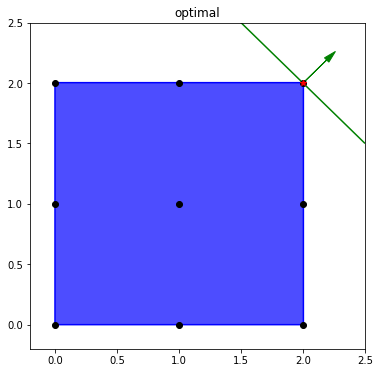
\includegraphics[width=2.5cm]{figures/optimal.png}
  \end{minipage} &
    \begin{tabular}{rr}
$\text{Max: }$ & $x + y$\\
 $\text{Such that: }$ & $0\leq x \leq 2$\\
  & $0\leq y \leq 2$\\
  & $x,y \in \mathbb{Z}$
    \end{tabular}
\end{tabular}
\subsubsection{Multiple optimal solution}
Optimal value is attained at more than one point of the feasible region.

\begin{tabular}{lc}
  \begin{minipage}{2.5cm}
    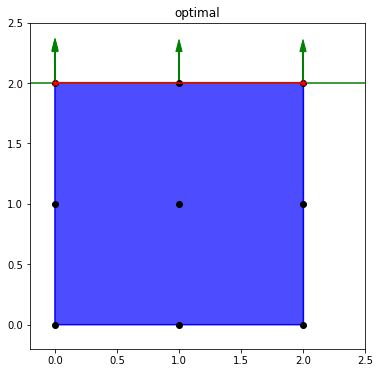
\includegraphics[width=2.5cm]{figures/optimal_multiple.png}
  \end{minipage} &
    \begin{tabular}{rr}
$\text{Max: }$ & $y$\\
 $\text{Such that: }$ & $0\leq x \leq 2$\\
  & $0\leq y \leq 2$\\
  & $x,y \in \mathbb{Z}$
    \end{tabular}
\end{tabular}

\subsubsection{Infeasible}
Feasible region is empty: it is impossible to satisfy all the constraints simultaneously.

\begin{tabular}{lp{5cm}}
  \begin{minipage}{2.5cm}
    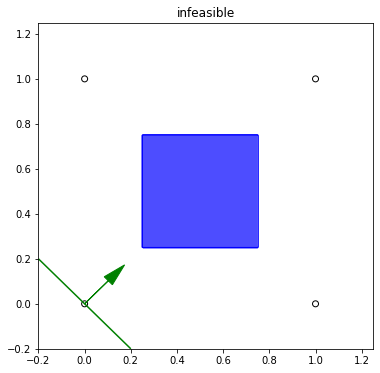
\includegraphics[width=2.5cm]{figures/infeasible.png}
  \end{minipage} &
    \begin{tabular}{rr}
$\text{Max: }$ & $x+y$\\
 $\text{Such that: }$ & $1\leq 4 x \leq 3$\\
  & $1 \leq 4 y \leq 3$\\
  & $x,y \in \mathbb{Z}$
    \end{tabular}

  (the feasible region of the \emph{relaxed} problem is shown in blue)
\end{tabular}

\subsubsection{Unbounded}
Feasible region is unbounded, and furthermore, the objective function can be optimized indefinitely.

\begin{tabular}{lc}
  \begin{minipage}{2.5cm}
    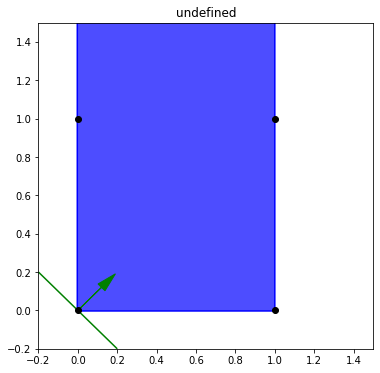
\includegraphics[width=2.5cm]{figures/unbounded_integer.png}
  \end{minipage} &
    \begin{tabular}{rr}
$\text{Max: }$ & $x+y$\\
 $\text{Such that: }$ & $0\leq x \leq 1$\\
  & $0\leq y$\\
  & $x,y \in \mathbb{Z}$
    \end{tabular}
\end{tabular}

\subsubsection{Unbounded region, but with optimal value}
It is possible that the feasible region is unbounded, but there is a finite optimal value (unique or multiple):
\begin{tabular}{lc}
  \begin{minipage}{2.5cm}
    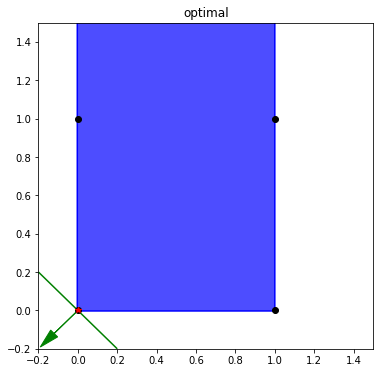
\includegraphics[width=2.5cm]{figures/unbounded_region_optimal_problem.png}
  \end{minipage} &
    \begin{tabular}{rr}
$\text{Min: }$ & $x+y$\\
 $\text{Such that: }$ & $0\leq x \leq 1$\\
  & $0\leq y$\\
  & $x,y \in \mathbb{Z}$
    \end{tabular}
\end{tabular}

% \subsubsection{Undefined}
% The feasible region for the relaxed problem is unbounded, and there is no optimal value, but the software will not waste resources deciding whether the feasible region is empty or unbounded, since it may not be easy to decide if there are integer points in the region:
% \begin{tabular}{lc}
%   \begin{minipage}{2.5cm}
%     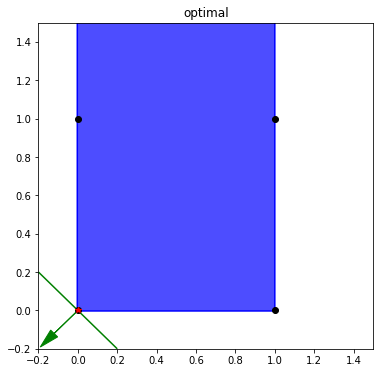
\includegraphics[width=2.5cm]{figures/unbounded_region_optimal_problem.png}
%   \end{minipage} &
%     \begin{tabular}{rr}
% $\text{Max: }$ & $y$\\
%  $\text{Such that: }$ & $0\leq x \leq 2$\\
%   & $0\leq y$\\
%   & $x,y \in \mathbb{R}$
%     \end{tabular}
% \end{tabular}
\subsection{The Backpack Problem}
Choose several items from a list, that fit into our backpack, and so that their total value is maximized
\begin{tabular}{r|r|r}
  Item & Weight & Value\\
  \hline
  $I_1$ & $ w_1$ & $v_1$\\
  $\dots$ & $\dots$ & $\dots$\\
  $I_n$ & $ w_n$ & $v_n$\\
\end{tabular}
\subsubsection{Decision variables}
$$x_j=\left\{\begin{array}{ll}
  1 & \text{put item } j \text{ in backpack}\\
  0 & \text{do not put item } j \text{ in backpack}
\end{array}\right. $$
\subsubsection{Objetive}
Maximize total value, only items in the backpack contribute:
$$\text{Max: } \sum_{j=1}^n x_j v_j$$
\subsubsection{Constraints}
All $x_j$ are either $0$ or $1$, and they fit in the backpack:
\begin{tabular}{rcl}
$\sum_{j=1}^n x_j w_j$ &$\leq$& $\text{ backpack capacity}$\\
$0$&$\leq$&$ x_j$, for $j=1,\dots,n$\\
$x_j$&$\leq$&$ 1$, for $j=1,\dots,n$\\
$x_j$&$\in$&$ \mathbb{Z}$, for $j=1,\dots,n$
\end{tabular}

\subsection{\texttt{optlang}}
{\tiny
\lstinputlisting[language=python]{optlang.py}
}

\end{multicols*}
\end{document}
